\documentclass[10pt]{article}
\usepackage[margin=0.9in]{geometry}
\usepackage{amsmath,amssymb}
\usepackage{booktabs}
\usepackage{array}
\usepackage{xcolor}
\usepackage{graphicx}
\usepackage{parskip}
\usepackage{listings}
\usepackage{enumitem}
\usepackage{needspace}
\usepackage[most]{tcolorbox}
\usepackage[colorlinks=true,linkcolor=blue!60!black,urlcolor=blue!60!black,citecolor=blue!60!black]{hyperref}

\definecolor{cset}{RGB}{31,111,184}     % a set (entities)
\definecolor{cfield}{RGB}{46,139,79}    % a field
\definecolor{cop}{RGB}{192,82,42}       % an operator (a step)
\definecolor{cwhere}{RGB}{154,125,26}   % the locating word of the math pane
\definecolor{cmuted}{gray}{0.45}

\lstdefinestyle{sh}{basicstyle=\ttfamily\scriptsize,frame=single,backgroundcolor=\color{gray!6},
  columns=fullflexible,breaklines=true,keepspaces=true,showstringspaces=false}
\renewcommand{\topfraction}{0.95}\renewcommand{\bottomfraction}{0.6}\renewcommand{\textfraction}{0.05}\renewcommand{\floatpagefraction}{0.75}
\newcommand{\code}[1]{\texttt{#1}}
\newcolumntype{P}[1]{>{\raggedright\arraybackslash}p{#1}}

% ------------------------------------------------------------------------------------------------
% THE TWO PANE TEMPLATES, after the two panes of the Plexus watcher. The PLEXUS pane says what a
% model IS: a headline, a few sentences, the entities, then every step of the loop in story order,
% each with its kind's glyph, a plain name and one line. The MATH pane shows every equation of the
% run at once, in one notation, a locating word to the right of each, then one legend of the
% variables and one of the constants.
% ------------------------------------------------------------------------------------------------
\newtcolorbox{plexuspane}[2][]{enhanced,breakable,colback=gray!4,colframe=gray!60,boxrule=0.5pt,arc=2pt,
  left=6pt,right=6pt,top=4pt,bottom=4pt,fonttitle=\small,coltitle=black,colbacktitle=gray!16,
  title={\textsc{plexus pane}\quad\textbf{#2}},#1}
\newtcolorbox{mathpane}[2][]{enhanced,breakable,colback=white,colframe=gray!60,boxrule=0.5pt,arc=2pt,
  left=6pt,right=6pt,top=4pt,bottom=4pt,fonttitle=\small,coltitle=black,colbacktitle=gray!16,
  title={\textsc{math pane}\quad\textbf{#2}},#1}
\newcommand{\pset}[3]{\item[\textcolor{cset}{\large$\bullet$}] \textbf{#1} {\color{cmuted}(#2)} --- #3}
\newcommand{\pfield}[3]{\item[\textcolor{cfield}{$\blacksquare$}] \textbf{#1} {\color{cmuted}(#2)} --- #3}
\newcommand{\pstep}[4]{\item[\textcolor{cop}{#1}] \textbf{#2} {\color{cmuted}\code{#3}} --- #4}
\newcommand{\kseed}{$\circ$}            % seed: once, before dynamics
\newcommand{\klat}{$\leftrightarrow$}   % lateral: within a set
\newcommand{\kexch}{$\rightleftarrows$} % exchange: set <-> field
\newcommand{\kfield}{$\boxdot$}         % field: field -> field
\newcommand{\kcall}{$\ast$}             % the prototype's per-frame callback, not a spec operator
\newcommand{\pheadline}[1]{{\normalsize\bfseries #1}\par\medskip}
\newcommand{\pentities}{\par\textcolor{cwhere}{\textsc{entities}}\par\nopagebreak}
\newcommand{\psteps}{\par\medskip\textcolor{cwhere}{\textsc{gnn} --- the steps, in story order}\par\nopagebreak}
\newenvironment{pitems}{\begin{itemize}[leftmargin=1.6em,itemsep=1pt,topsep=2pt]}{\end{itemize}}
\newenvironment{meqs}{\par\begin{tabular}{@{}p{0.74\linewidth}>{\color{cwhere}\bfseries\small}p{0.22\linewidth}@{}}}{\end{tabular}\par}
\newcommand{\meq}[2]{$\displaystyle #1$ & #2 \\[7pt]}
\newcommand{\mvariables}{\par\smallskip\textcolor{cwhere}{\textsc{variables}}\par\nopagebreak}
\newcommand{\mconstants}{\par\smallskip\textcolor{cwhere}{\textsc{constants}}\par\nopagebreak}
\newenvironment{mlegend}{\begin{tabular}{@{}>{$}l<{$}@{\quad}P{0.80\linewidth}@{}}}{\end{tabular}}
\newcommand{\msym}[2]{#1 & #2 \\}

\title{\textbf{Per-cell active-strain fit}}
\author{C. Allier --- HHMI Janelia Research Campus}
\date{}

\begin{document}
\maketitle

\noindent Companion to \href{https://github.com/allierc/GNN_MPM_cardio}{\code{github.com/allierc/GNN\_MPM\_cardio}}.
\S\ref{sec:data} the data and the cell segmentation; \S\ref{sec:model} the model; \S\ref{sec:mpm} the material
point method; \S\ref{sec:pulse} how the pulse drives the cells; \S\ref{sec:results} results; \S\ref{sec:run} install and run.

%================================================================================================
\section{Data}\label{sec:data}

\textbf{Recordings.} Two confluent sheets of human iPSC-derived cardiomyocytes on a 15~kPa gel,
phase contrast, $2048\times2048$~px, 24 frames per second (41.7~ms per frame): one healthy
(239 frames), one carrying a hypertrophic cardiomyopathy (HCM) mutation (299 frames). No electrical recording, no calcium dye, no stain, no force
measurement.


\textbf{Tracking (the ``grid flow'').} Each movie is tracked on a $137\times137$ lattice of points
15~px apart (18,769 points), giving the point positions $x_i(t)$ in image pixels, referenced to frame~0
(Lagrangian). Displacement amplitude: mean 1.7~px, maximum $\approx$15~px (healthy); mean 2.8~px (HCM).
The sheet domain in the engine is $x^{\rm world} = 0.15 + 0.70\,x^{\rm img}/2048$. Shipped as
\code{data/\{healthy,hcm\}/grid\_flow.npz} with a sha256 of the array checked at load.

\textbf{Cell segmentation} (\code{cardio/segmentation.py}, \code{cardio/seg/}; Figs.~\ref{fig:steps} and \ref{fig:data}). The pixels of one
cell move together, so the cells can be found from the motion alone: the tracking nodes of one cell contract along the
same direction, and a border lies where that direction changes between neighbouring nodes. The same procedure is
used on the healthy and the HCM recording.
\begin{enumerate}[leftmargin=1.6em,itemsep=1pt]
\item \emph{Borders from the motion.} The contraction direction of each node is read from its trajectory averaged
over the beats; borders are where this direction, smoothed over the lattice, changes sharply.
\item \emph{Nuclei.} One dark nucleus per cell is found on the rest frame (flat-fielded with a 60-px blur, then
Laplacian-of-Gaussian blobs of 25--60~px): 472 for the healthy sheet, 434 for HCM; each is the seed of one cell.
\item \emph{Watershed.} Seeded by the nuclei, on the border strength plus the distance to the nearest seed, every
node is given one cell: 472 (434) cells.
\item \emph{Label image.} For the engine, a $2560\times2560$ map in which each pixel takes the label of the nearest
node.
\end{enumerate}

\begin{figure}[!ht]
\centering
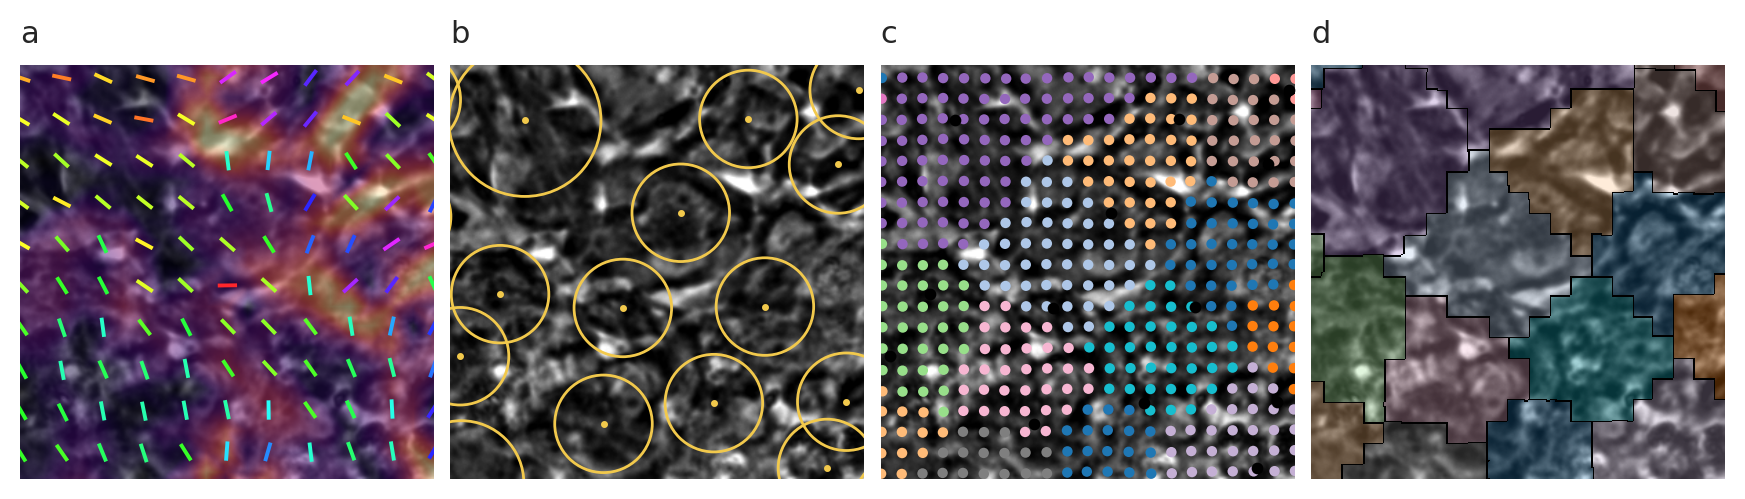
\includegraphics[width=1.0\linewidth]{figures/fig_steps.png}
\caption{Segmentation on a $300\times300$~px detail of the healthy rest frame. (a) Borders from the motion: contraction
axis of every second node (colour = angle) over the border strength (bright = border). (b) Nuclei. (c) Watershed: nodes
coloured by cell, seeds in black. (d) The engine's label image, as outlines.}
\label{fig:steps}
\end{figure}

\begin{figure}[t]
\centering
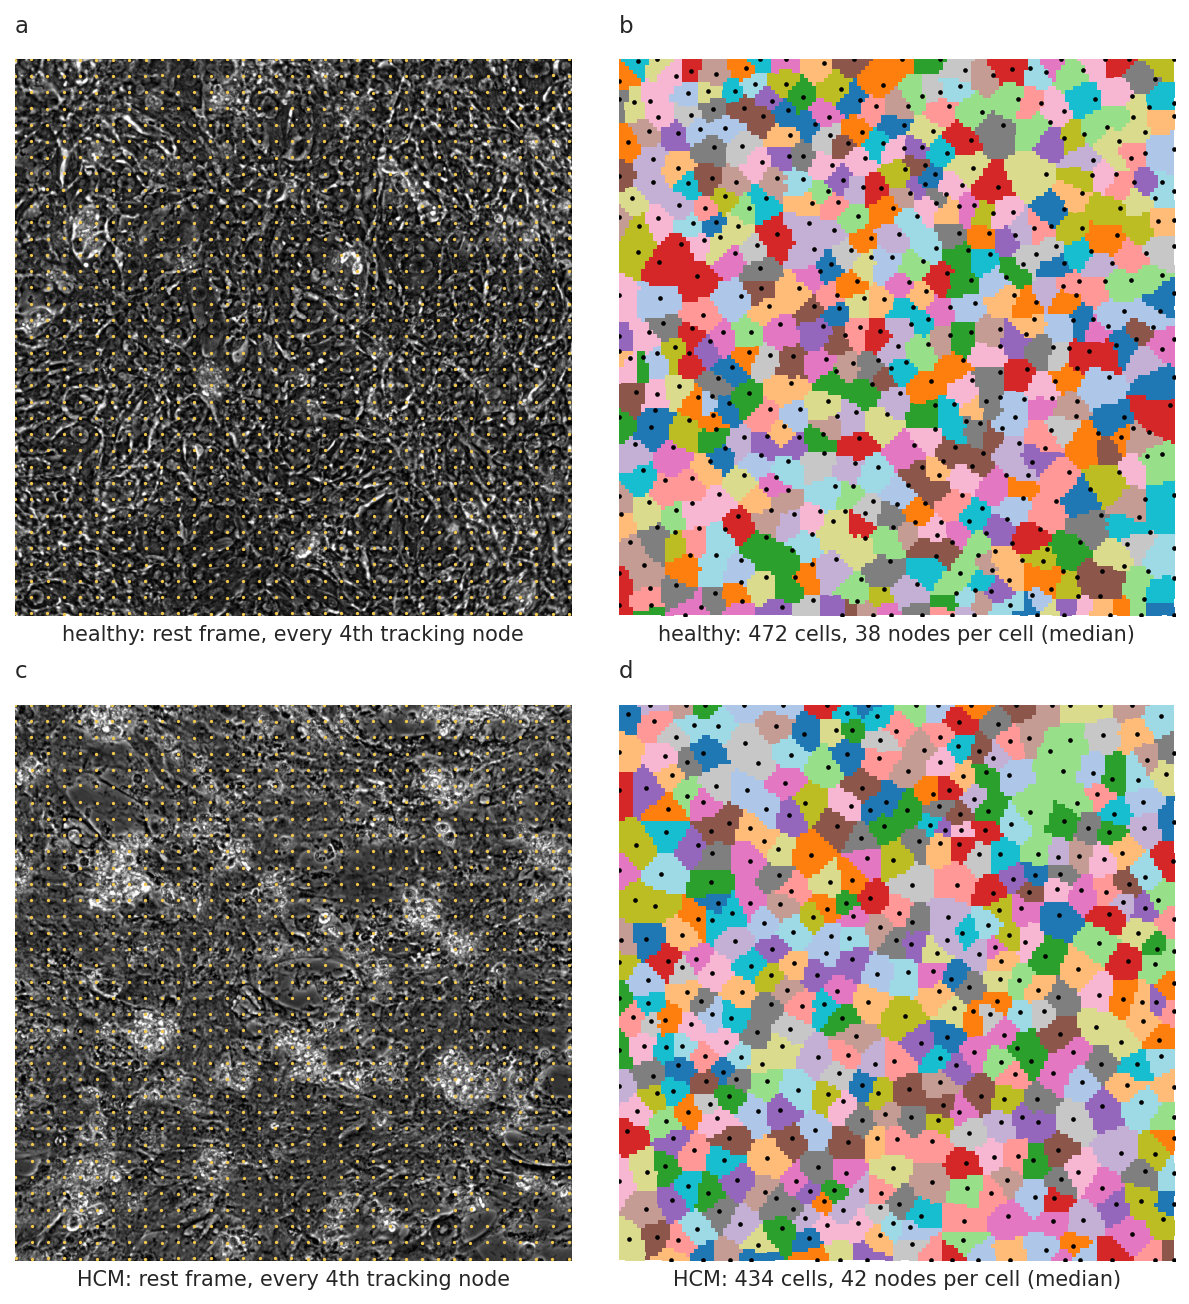
\includegraphics[width=\linewidth]{figures/fig_data.png}
\caption{The data. (a, c) Rest frame of the healthy and HCM recordings with every 4th node of the tracking lattice.
(b, d) The segmentation on the lattice, one colour per cell, nuclei in black.}
\label{fig:data}
\end{figure}



\clearpage
%================================================================================================
\section{The model}\label{sec:model}

Every segmented cell is modelled as a patch of elastic material that shortens along its own fibre axis when a shared
activation pulse reaches it, and is subject to a drag and a spring (see details below); gradient descent through the
simulation returns the per-cell numbers that make the simulated sheet move like the recording, cell by cell.

The sheet is cut into the 472 segmented cells (434 for HCM), each filled with 120 material points. One step of
the simulation is one recorded frame: $dt = 0.002$ engine time units, 41.7~ms of recording. In each step the engine
first computes two accelerations on every point, a drag and a spring, from the state at the start of the step.
It then runs 10 sub-steps of $dt = 2\times10^{-4}$ of the material point method (\S\ref{sec:mpm}). The sub-steps
take the points' positions, velocities, deformations and stiffnesses together with the two accelerations, and
return new positions, velocities and deformations. Drag and spring are not recomputed inside the sub-steps: the
same two accelerations act in all ten sub-steps. After the ten sub-steps, once per frame, every cell is shortened along its fibre axis in proportion to its activation
(\S\ref{sec:pulse}), and each cell is measured: the least-squares affine map of its points from their rest positions,
$A_j$ (a $2\times2$ matrix, the cell's mean deformation gradient: stretch, shear and rotation) and $u_j$ (the shift of
its centroid). The function \code{cell\_affine} (\code{cardio/recording.py}) computes it, identically for the model's
material points and for the recording's tracking nodes. It is what the fit is trained on: the loss is the mean squared
mismatch of $A_j$ and $u_j$ between model and recording, each scaled by the recording's own spread.

\textbf{Drag} (operator \code{drag}, \code{operators/motion\_ops.py}). Viscous friction: a point of velocity $v$ gets
the acceleration $-k\,v$, with $k = 150$ per engine time unit, so a point loses 63\% of its speed in 3.3 frames. It
stands for friction against the surroundings. Without it the sheet rings on its spring. With a weaker drag ($k = 30$), a step in the activation made the sheet overshoot to $-32$\% of its plateau
and stay 10\% off twenty frames later. At $k = 150$ the drag is 0.75 of the value that would critically damp the
spring ($2\sqrt{\kappa}$, with $\kappa$ below).

\textbf{Spring} (operator \code{anchor\_percell}, \code{cardio/ops\_percell.py}). The cells sit on a 15~kPa gel,
and every material point is attached to its own rest position $X$ by a spring. A point displaced to $x$ is pulled
back with the acceleration $\kappa\,(X - x)$, where $\kappa$ is the spring stiffness: $\kappa = 10^4$ in engine units times a factor learned per cell. The
$10^4$ is set by hand and not trained. The factor starts at 1, is held near 1 by a penalty and may range from 0.14 to
7.4; after training it lies between 0.89 and 1.19 (healthy). It stands for the cells' adhesion to the gel. Without it the whole sheet
relaxes through the drag alone, an estimated 460 frames at $k = 150$ (90 at $k = 30$), against a beat of 55--65
frames.

%================================================================================================
\section{Material point method}\label{sec:mpm}

The material point method (MPM) of Sulsky et al.\ \cite{sulsky1994} simulates a continuum with particles that carry mass,
velocity and deformation, coupled through a background grid; we use its moving-least-squares form (MLS-MPM) of
Hu et al.\ \cite{hu2018}. Our PyTorch implementation is \url{https://github.com/saalfeldlab/MPM_pytorch}.

\textbf{Implementation.} Each step is one operator (\code{mpm\_strain}, \code{mpm\_scatter}, \code{mpm\_grid\_update},
\code{mpm\_gather}); the four run together as the sub-step block, in their \code{differentiable} implementation after
Xu et al.\ \cite{xu2025}: the same arithmetic as the default bodies, with each result bound to a new tensor so that
automatic differentiation keeps what the backward pass needs. The grid has 128 by 128 nodes over the unit square; each
point reaches the 3 by 3 nodes nearest to it, with quadratic B-spline weights. The drag and spring accelerations of
\S\ref{sec:model} enter in the second step, as a body force; the pulse of \S\ref{sec:pulse} enters in the first step, as
a change of the deformation gradient written once per frame, which the second step turns into stress.

\textbf{The four steps,} in the order they run in each of the 10 sub-steps.
\begin{enumerate}[leftmargin=1.6em,itemsep=4pt]
\item \textbf{Advance the strain} (\code{mpm\_strain}). Each point updates its deformation from the velocity
gradient it carries, then the material rule is applied: elastic keeps the deformation as updated (this model); a
liquid would keep only the volume; a plastic material (snow) would clip the singular values of $F$; a
viscoelastic one would let $F$ relax toward the current shape over a time constant.
\[ F_p \leftarrow (I + \Delta t\, C_p)\, F_p, \qquad J_p = \det F_p \]
\item \textbf{Points to grid} (\code{mpm\_scatter}). Each point computes its stress from its deformation, then
spreads its mass, its momentum and the impulse of its stress onto the 9 nearest nodes, weighted by $w_{np}$. The
stress impulse points back toward the rest shape. The drag and spring accelerations are added here, clamped.
\begin{align*}
\sigma_p &= 2\mu_p\,(F_p - R_p)\,F_p^{\!\top} + \lambda_p\,(J_p - 1)\,J_p\, I \\
m_n &= \sum_p w_{np}\, m_p \\
p_n &= \sum_p w_{np}\Big[ m_p\big(v_p + C_p (x_n - x_p)\big) - \frac{4\Delta t}{\Delta x^2}\, V_p\, \sigma_p\,(x_n - x_p) + \Delta t\, m_p\, \bar a_p \Big] \\
\bar a_p &= \mathrm{clamp}\big(-k\, v_p + \kappa_p (X_p - x_p),\ \pm a_{\max}\big)
\end{align*}
\item \textbf{Solve the grid} (\code{mpm\_grid\_update}). Each node turns its momentum into a velocity; the wall
condition is applied at the box faces.
\[ v_n = \frac{p_n}{m_n}\ \ (m_n > 0,\ \text{else } 0), \qquad v_n \leftarrow \mathrm{BC}(v_n, x_n) \]
\item \textbf{Grid to points} (\code{mpm\_gather}). Each point takes the velocity and the velocity gradient of the
nodes around it, and moves.
\[ v_p = \sum_n w_{np}\, v_n, \qquad C_p = \frac{4}{\Delta x^2}\sum_n w_{np}\, v_n\,(x_n - x_p)^{\!\top}, \qquad x_p \leftarrow x_p + \Delta t\, v_p \]
\end{enumerate}
The weight of node $n$ at point $p$ is a product of one-dimensional quadratic B-splines:
\[ w_{np} = \prod_{d=1}^{2} N\!\left(\frac{x_{n,d} - x_{p,d}}{\Delta x}\right), \qquad
   N(r) = \begin{cases} \tfrac34 - r^2 & |r| < \tfrac12 \\ \tfrac12\left(\tfrac32 - |r|\right)^2 & \tfrac12 \le |r| < \tfrac32 \\ 0 & \text{else}\end{cases} \]

\begin{center}\small
\begin{tabular}{@{}>{$}l<{$}P{0.78\linewidth}@{}}
\toprule
\text{symbol} & meaning \\
\midrule
F_p,\ R_p,\ J_p & deformation gradient of point $p$, its rotation part ($F = R\,S$ with $S$ the stretch), its determinant \\
\sigma_p & stress of point $p$ in the fixed-corotated law: $\mu$ penalises change of shape ($F - R$), $\lambda$ change of volume ($J - 1$); a rotation alone gives none \\
C_p & velocity gradient carried by point $p$ \\
x_p,\ v_p,\ X_p & position, velocity and rest position of point $p$ \\
m_p,\ V_p & mass and rest volume of point $p$; $m_p = \rho V_p$ with density $\rho = 1$ \\
m_n,\ p_n,\ v_n,\ x_n & mass, momentum, velocity and position of grid node $n$ \\
w_{np} & weight of node $n$ at point $p$, over the 3 by 3 nodes around the point \\
\bar a_p & acceleration of point $p$ from drag and spring, clamped at $a_{\max} = 200$ \\
\mu_p,\ \lambda_p & Lam\'e stiffnesses of the point's cell: $\mu = E/2(1+\nu)$, $\lambda = E\nu/(1+\nu)(1-2\nu)$, $E$ the Young's modulus, $\nu = 0.3$ \\
\Delta t,\ \Delta x & sub-step $2\times10^{-4}$ engine time units; grid spacing $1/128$ of the unit square \\
k,\ \kappa_p & drag $150$ and spring stiffness of point $p$ ($10^4$ times the cell's learnable factor) \\
\mathrm{BC} & wall condition within 0.06 of a box face: the velocity into the wall is removed, the rest damped by 0.5; the sheet never reaches it \\
\bottomrule
\end{tabular}
\end{center}
The sub-step stays below the stability limit $\Delta t < \Delta x / \sqrt{E/\rho}$: $8.7\times10^{-4}$ against
$2\times10^{-4}$ for the starting Young's modulus $E = 80$.

%================================================================================================
\section{Pulse activation}\label{sec:pulse}

Nothing in \S\ref{sec:mpm} makes a cell move on its own: the material point method only relaxes elastic stress.
The beat enters as a change of each cell's rest shape, once per frame, written into the deformation gradient of
the cell's points, and the material law of \S\ref{sec:mpm} turns it into motion during the following sub-steps.

\textbf{The shared pulse.} One activation curve $\gamma(t)$, $t$ the frame inside the beat (41.7~ms each; 57
frames per beat for the healthy sheet, 65 for HCM), a sigmoid rise and fall normalised to start at zero:
\[ s(t) = \mathrm{sig}\!\left(\frac{t - t_0}{\tau_r}\right)\,\mathrm{sig}\!\left(\frac{t_0 + d - t}{\tau_d}\right), \qquad
   \gamma(t) = \frac{s(t) - s(0)}{1 - s(0)}, \qquad \mathrm{sig}(x) = \frac{1}{1 + e^{-x}} . \]
Its four numbers (onset $t_0$, rise time $\tau_r$, plateau $d$, decay time $\tau_d$) are learned, starting from a
least-squares fit to the recording's mean shortening curve. The pulse does not travel: the recording's onsets
show no correlation with position ($r \approx 0$), so every cell reads the same clock. In a rollout over several
beats the same $\gamma$ fires again at each recorded onset; nothing is reset between beats.

\textbf{Each cell's own timing.} Cell $j$ reads the pulse shifted by its delay $\delta_j$ and with its own rise,
plateau and decay, and adds two shared temporal modes with its own weights:
\[ \gamma_j(t) = \left[\frac{s_j(t - \delta_j) - s_j(-\delta_j)}{1 - s_j(-\delta_j)}\right]_+ + \sum_{k=1}^{2} a_{jk}\,\psi_k(t),
   \qquad \text{clamped to } [0, 1.5], \]
where $s_j$ is $s$ with $\tau_r e^{u_{r,j}}$, $d\, e^{u_{d,j}}$, $\tau_d e^{u_{\tau,j}}$ in place of $\tau_r$, $d$,
$\tau_d$. The modes $\psi_k(t)$ are one number per frame, shared by the sheet, with $\psi_k(0) = 0$; their frame
steps and the weights are penalised, as are the per-cell logs $u$ (zero = the shared pulse). The recording asks for
this: its beat is 88\% one time course, 6.7\% a second (early-negative, late-positive: cells lead or lag) and 3\% a
third, and the per-cell peak frames spread over 14 frames (0.6~s) with no spatial gradient.

\textbf{Injection into the material.} At the end of every frame $t$ (after its ten sub-steps, before the edge
band is pinned and the cells are measured), for every material point $p$ of cell $j$:
\[ F_p \leftarrow G_j(t)\,F_p, \qquad G_j(t) = I + c_j(t)\, f_j f_j^{\!\top} + c_{2j}(t)\, f_j^{\perp} f_j^{\perp\top}, \]
\[ c_j(t) = \frac{(\gamma_j(t) - \gamma_j(t-1))\, g_j}{1 + \gamma_j(t-1)\, g_j}, \qquad
   c_{2j}(t) = \frac{(\gamma_j(t) - \gamma_j(t-1))\, g_{2j}}{1 + \gamma_j(t-1)\, g_{2j}}, \]
with $f_j = (\cos\varphi_j, \sin\varphi_j)$ the fibre axis and $f_j^{\perp}$ its normal. The increments compound
exactly: after any number of frames the active factor along the fibre is $1 + \gamma_j(t)\,g_j$, so the total active
deformation at activation $\gamma_j$ is $I + \gamma_j\,(g_j f_j f_j^{\!\top} + g_{2j} f_j^{\perp} f_j^{\perp\top})$.
The deformation gradient now reads the cell's material as stretched by $1 + \gamma_j g_j$ along its fibre although
no point has moved, so the stress of \S\ref{sec:mpm} step~2, $2\mu_p (F_p - R_p) F_p^{\!\top}$, pulls the cell's
points together along $f_j$ until that stretch is undone: the cell's rest length along its fibre is divided by
$1 + \gamma_j g_j$, a shortening of about $\gamma_j g_j$ ($g_j$ 0.037 median, healthy), realised at about 60\%
against the pull of the neighbours and the substrate spring. Across the fibre the same with $g_{2j}$: a negative
$g_{2j}$ widens the cell, and the fits return $g_{2j}/g_j \approx -0.7$, near area preservation. This is the
active-strain form $F = F_e F_a$, $F_e$ the elastic part and $F_a = G^{-1}$ the active one: the pulse moves the rest
shape, the elasticity moves the points.

\begin{center}\small
\begin{tabular}{@{}>{$}l<{$}P{0.78\linewidth}@{}}
\toprule
\text{symbol} & meaning \\
\midrule
\gamma(t),\ s(t) & the shared pulse (0 at rest, about 1 at full activation) and its unnormalised sigmoid product \\
t_0,\ \tau_r,\ d,\ \tau_d & onset frame, rise time, plateau duration and decay time of the pulse, in frames; learned, 4 numbers per sheet \\
\gamma_j(t) & activation of cell $j$ at frame $t$; $[\,\cdot\,]_+$ the positive part \\
\delta_j & delay of cell $j$, in frames (bounded to $\pm 8$) \\
u_{r,j},\ u_{d,j},\ u_{\tau,j} & cell $j$'s log factors on the rise time, plateau and decay time; 0 = the shared pulse \\
\psi_k(t),\ a_{jk} & the two shared temporal modes (one number per frame, 0 at frame 0) and cell $j$'s weight on each \\
g_j,\ g_{2j} & active strain of cell $j$ along and across its fibre at full activation \\
f_j,\ f_j^{\perp},\ \varphi_j & fibre axis of cell $j$, its in-plane normal, and the axis angle \\
G_j(t),\ c_j,\ c_{2j} & the frame's active increment on the deformation gradient of cell $j$'s points, and its two coefficients \\
F_p,\ R_p,\ \mu_p & deformation gradient and rotation of point $p$, and its shear stiffness (\S\ref{sec:mpm}) \\
\bottomrule
\end{tabular}
\end{center}

%================================================================================================
\section{Results}\label{sec:results}

\textbf{Learnables.} The model learns principally four parameters per cell:
\begin{enumerate}[leftmargin=1.6em,itemsep=1pt]
\item \textbf{the strain}: $g_j$ along the fibre at full activation and $g_{2j}$ across it. The realised
shortening is about 60\% of $g$ (healthy). Adding $g_2$ raised the explained variance of the per-cell strain
maps from 0.69 to 0.82;
\item \textbf{its direction}: $\varphi_j$, inferred from motion alone; moved by the fit by a median of
$10^\circ$ from its starting value;
\item \textbf{a gain}: $E_j$ (stiffness) and $\kappa_j$ (adhesion to the gel), both shrunk toward uniform;
\item \textbf{a pulse} (\S\ref{sec:pulse}): the shared $\gamma(t)$ (4 numbers) and per cell its delay $\delta_j$, three
time-course scalings and two mode weights.
\end{enumerate}
In numbers, the fit returns 5,311 for the healthy sheet and 4,909 for the HCM sheet: eleven per cell (472 and 434
cells; every cell carries them, the loss reads the 331 and 298 interior ones of \S\ref{sec:data}) and 119 and 135
shared by the sheet. Nothing else is learned: the drag $k$, the Poisson ratio $\nu$, the hand-set spring scale
$10^4$, the segmentation and the starting state are fixed.
\begin{center}\small
\begin{tabular}{@{}>{$}l<{$}lcP{0.50\linewidth}@{}}
\toprule
\text{symbol} & per & count (healthy / HCM) & what it is, and where it acts \\
\midrule
g_j & cell & 472 / 434 & active strain along the fibre at full activation: the shortening of \S\ref{sec:model}, applied once per frame as $I + \gamma_j(t)\,(g_j\, f_j f_j^{\!\top} + g_{2j}\, f_j^{\perp} f_j^{\perp\top})$ \\
g_{2j} & cell & 472 / 434 & active strain across the fibre (positive = thickening); 0 is the rank-1 model \\
\varphi_j & cell & 472 / 434 & fibre axis $f_j = (\cos\varphi_j, \sin\varphi_j)$ of the same strain \\
\log E_j & cell & 472 / 434 & Young's modulus of the cell, bound to its points as $\mu_p, \lambda_p$ (\S\ref{sec:mpm}, with $\nu = 0.3$); starts at $E = 80$ in the engine's own stress units, the value of the earlier recipes, not a kPa \\
\log\kappa_j & cell & 472 / 434 & factor on the substrate spring of the cell's points, $\kappa_p = 10^4\, e^{\log\kappa_0}\, e^{\log\kappa_j}$ (\S\ref{sec:model} spring, \S\ref{sec:mpm} $\bar a_p$) \\
\delta_j & cell & 472 / 434 & delay of the cell's activation, $\gamma_j(t) = \gamma(t - \delta_j)$ (\S\ref{sec:pulse}) \\
u_{r,j},\ u_{d,j},\ u_{\tau,j} & cell & $3\times$ 472 / 434 & log factors on the cell's rise time, plateau duration and decay time against the shared pulse's (\S\ref{sec:pulse}) \\
a_{j1},\ a_{j2} & cell & $2\times$ 472 / 434 & weights of the two shared temporal modes in the cell's activation, $\gamma_j(t) \mathrel{+}= \sum_k a_{jk}\,\psi_k(t)$ \\
\midrule
\gamma(t) & sheet & 4 / 4 & the shared pulse, a sigmoid rise and fall: onset $t_0$, rise time $\tau_r$, plateau $d$, decay time $\tau_d$ (\S\ref{sec:pulse}) \\
\log\kappa_0 & sheet & 1 / 1 & the sheet's substrate stiffness factor (fitted 0.93 of the hand-set value) \\
\psi_1(t),\ \psi_2(t) & sheet & $2\times 57$ / $2\times 65$ & the two temporal modes, one number per frame of the beat window (\S\ref{sec:pulse}) \\
\bottomrule
\end{tabular}
\end{center}

\textbf{Training.} The fit is run with Adam for 250 steps. Each family of parameters has its own step size
($g$ and $g_2$: 0.002; axis $\varphi$: 0.03; log stiffness: 0.06; shared pulse: 0.05; delay $\delta$: 0.1;
per-cell time-course and adhesion scalings: 0.05; temporal modes: 0.01, their weights: 0.02), decreasing along
a cosine to 5\% of its start. After every step the parameters are clipped to their bounds ($g \ge 0$,
$|g_2| \le 0.2$, $E_j$ within a factor 10 of 80, $|\delta| \le 8$ frames). The gradient is taken through every
sub-step of every beat's rollout; the starting state is not learned. Starting values: $g$ = the median peak
shortening of the recording, $\varphi$ = the axis of each cell's peak strain, the pulse = a least-squares fit
to the recording's mean shortening curve, every cell's Young's modulus $E_j = 80$ (engine stress units, \S\ref{sec:mpm}),
everything else zero. One fit takes 108~min
(healthy) and 144~min (HCM) on one RTX A6000; the loss falls from 1.78 to 0.19 and from 1.57 to 0.15.

\begin{figure}[!tb]
\centering
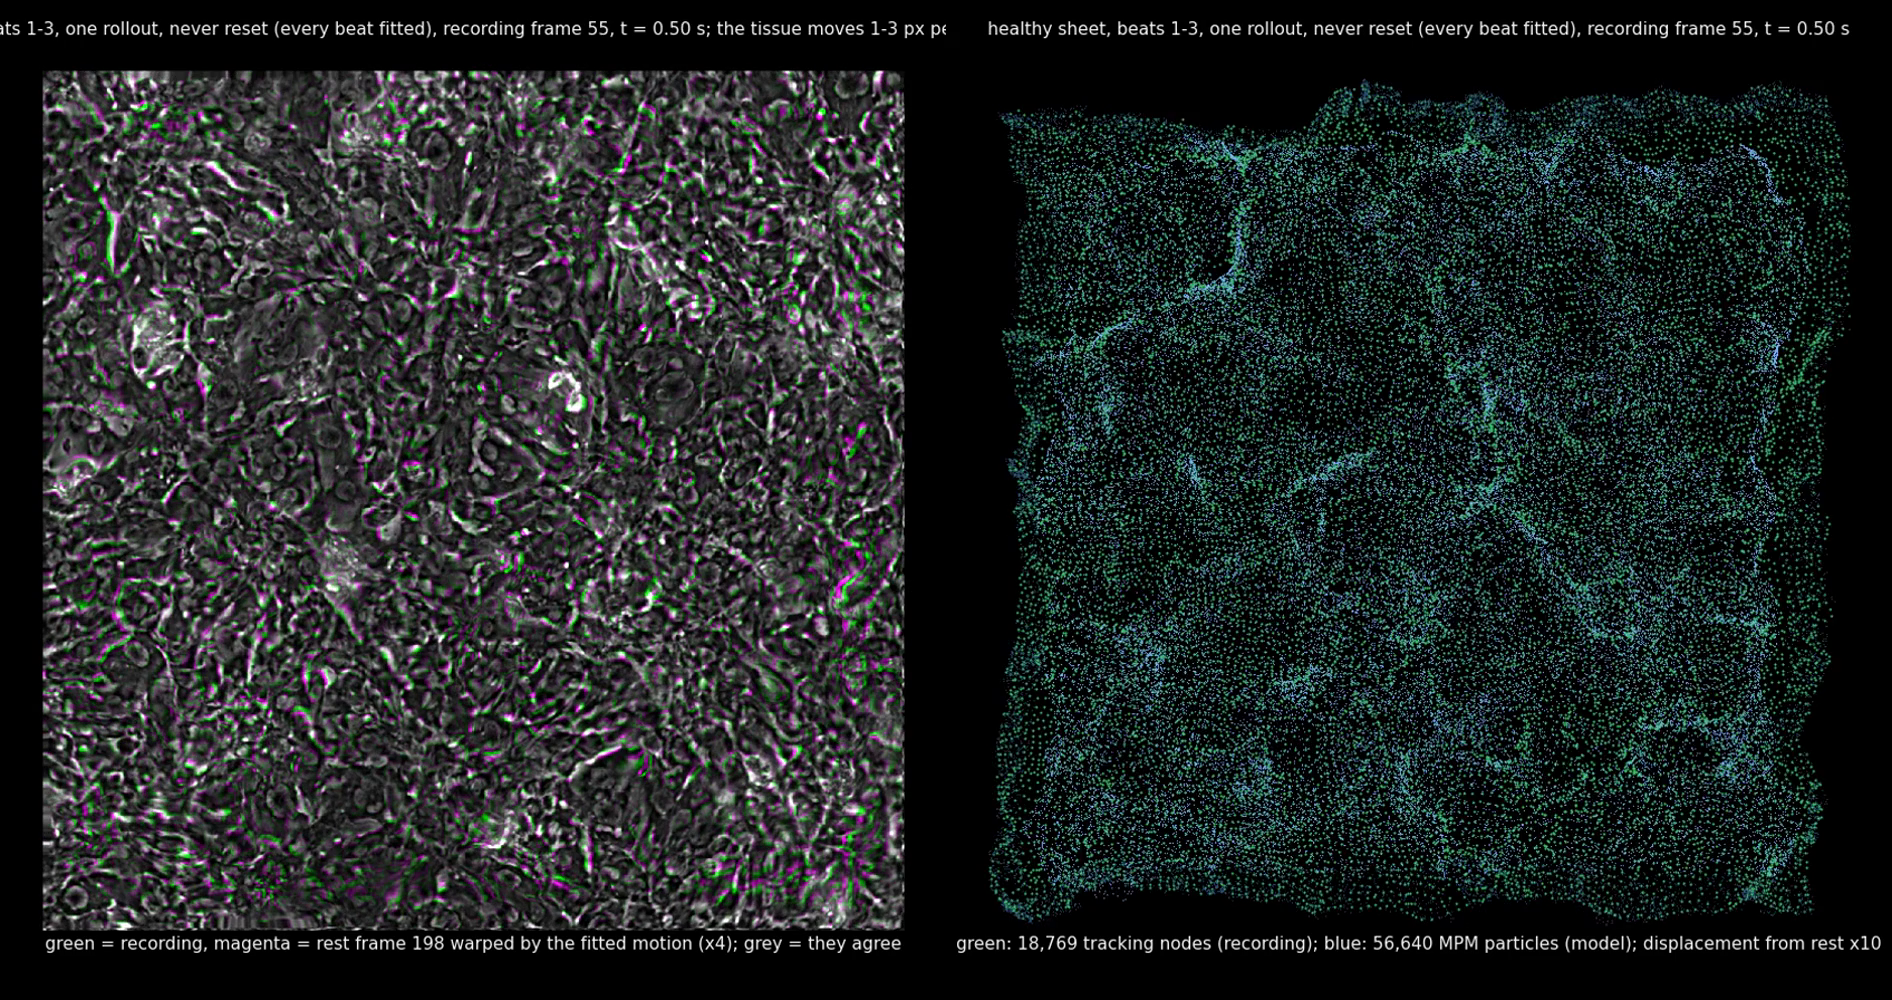
\includegraphics[width=0.86\linewidth]{figures/frame_overlay.png}
\caption{One frame of \code{docs/cont\_overlay\_particles.mp4} (made by \code{scripts/make\_cont\_overlay\_particles.sh},
\S\ref{sec:run}): the healthy sheet near peak contraction, beats 1--3 in one rollout that is never reset (every beat is
fitted). Left: the microscope frame in green and the rest frame warped by the fitted motion in magenta, motion drawn
$\times4$; grey where they agree. Right: the 18,769 tracking nodes (green) and the 56,640 material points (blue),
displacement from rest $\times10$.}
\label{fig:frame}
\end{figure}

\textbf{Reconstruction.} After optimisation the simulated sheet moves like the recording cell by cell
(Fig.~\ref{fig:frame}; Table~\ref{tab:fit}). One rollout through beats 1--3 without a reset explains
$R^2 = 0.849$ of the per-cell strain. The recording's own ceiling, from its singular value decomposition,
is 0.87 / 0.94 / 0.97 with one / two / three fixed spatial patterns. Two independent fits (another optimiser
seed and particle layout) agree per cell at $r = 0.90$--$0.92$ ($g$), $0.88$--$0.93$ ($g_2$), $0.83$--$0.88$
($\delta$), $7$--$10^\circ$ ($\varphi$); the median cell-to-cell difference is about one fifth of each map's
spread.

\begin{table}[h]
\centering\small
\begin{tabular}{@{}lcccc@{}}
\toprule
 & beat 1 & beat 2 & beat 3 & beat 4 \\
\midrule
healthy, $R^2$ strain maps $A$ & 0.870 & 0.872 & 0.871 & \\
healthy, $R^2$ displacements $u$ & 0.935 & 0.937 & 0.935 & \\
HCM, $R^2$ strain maps $A$ & 0.894 & 0.900 & 0.898 & 0.898 \\
HCM, $R^2$ displacements $u$ & 0.949 & 0.958 & 0.958 & 0.958 \\
\midrule
per-cell shortening correlation & \multicolumn{2}{c}{healthy 0.94} & \multicolumn{2}{c}{HCM 0.97} \\
replay of the fitted beat, $A$ / $u$ & \multicolumn{2}{c}{healthy 0.98 / 0.96} & \multicolumn{2}{c}{HCM 0.96 / 0.95} \\
\bottomrule
\end{tabular}
\caption{Quality of the reconstruction, from the fits rerun in this repository (\code{parity/runs/full\_repo\_healthy},
\code{parity/runs/full\_repo\_hcm}): $R^2$ against the recording per beat, for the per-cell strain maps $A$ and the
displacements $u$. Every beat is fitted: spread across beats 0.002 (healthy), 0.006 (HCM). The archived fits of
\code{reference/} give the same values to the third decimal.}
\label{tab:fit}
\end{table}

\Needspace{8\baselineskip}
The recording gives motion, not force, so the fit cannot separate a cell's stiffness from its active strain: a stiffer
cell that contracts harder, or a weaker contraction held for longer, moves the sheet the same way. On planted
parameters (the recording's rest-frame noise added, 3 seeds) the fit recovers $g$ to 0.10 of its spread ($r = 0.93$)
and $\varphi$ to $5^\circ$, but $\log E$ only to 0.40 ($r \approx 0.65$). On the real data the per-cell $E_j$, left
free, spreads over a factor of 200; the shrinkage $\lambda_E = 0.3$ holds it to $\pm12\%$ at a cost of 0.04 in
explained variance. The pulse length and the gain trade off likewise. The healthy / HCM differences of
Table~\ref{tab:sheets} therefore describe one dish of each under one prior, not a conclusion about the two conditions.

\begin{figure}[!tb]
\centering
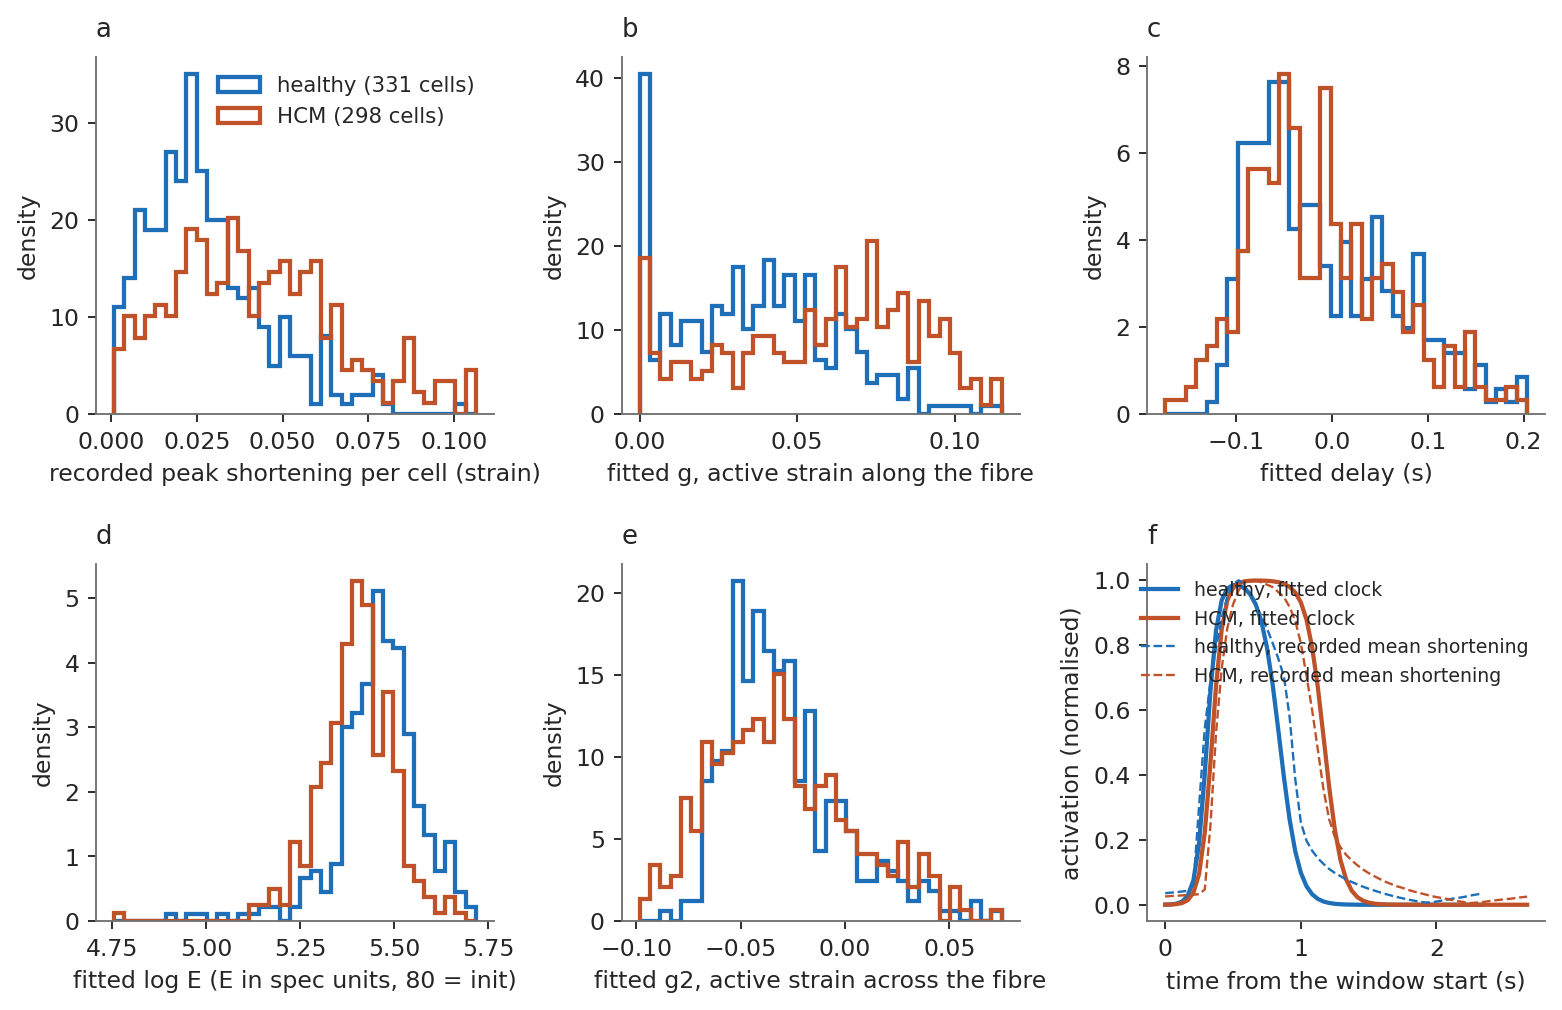
\includegraphics[width=0.96\linewidth]{figures/fig_sheets.png}
\caption{Healthy (blue, 331 cells) against HCM (red, 298 cells). (a) Peak shortening per cell read off the
recording. (b) Fitted $g$. (c) Fitted delay $\delta$ (s). (d) Fitted $\log E$ ($\lambda_E = 0.3$). (e) Fitted
$g_2$. (f) Fitted pulse $\gamma(t)$ of each sheet (solid) and recorded mean shortening, normalised (dashed).}
\label{fig:sheets}
\end{figure}

\begin{figure}[!tb]
\centering
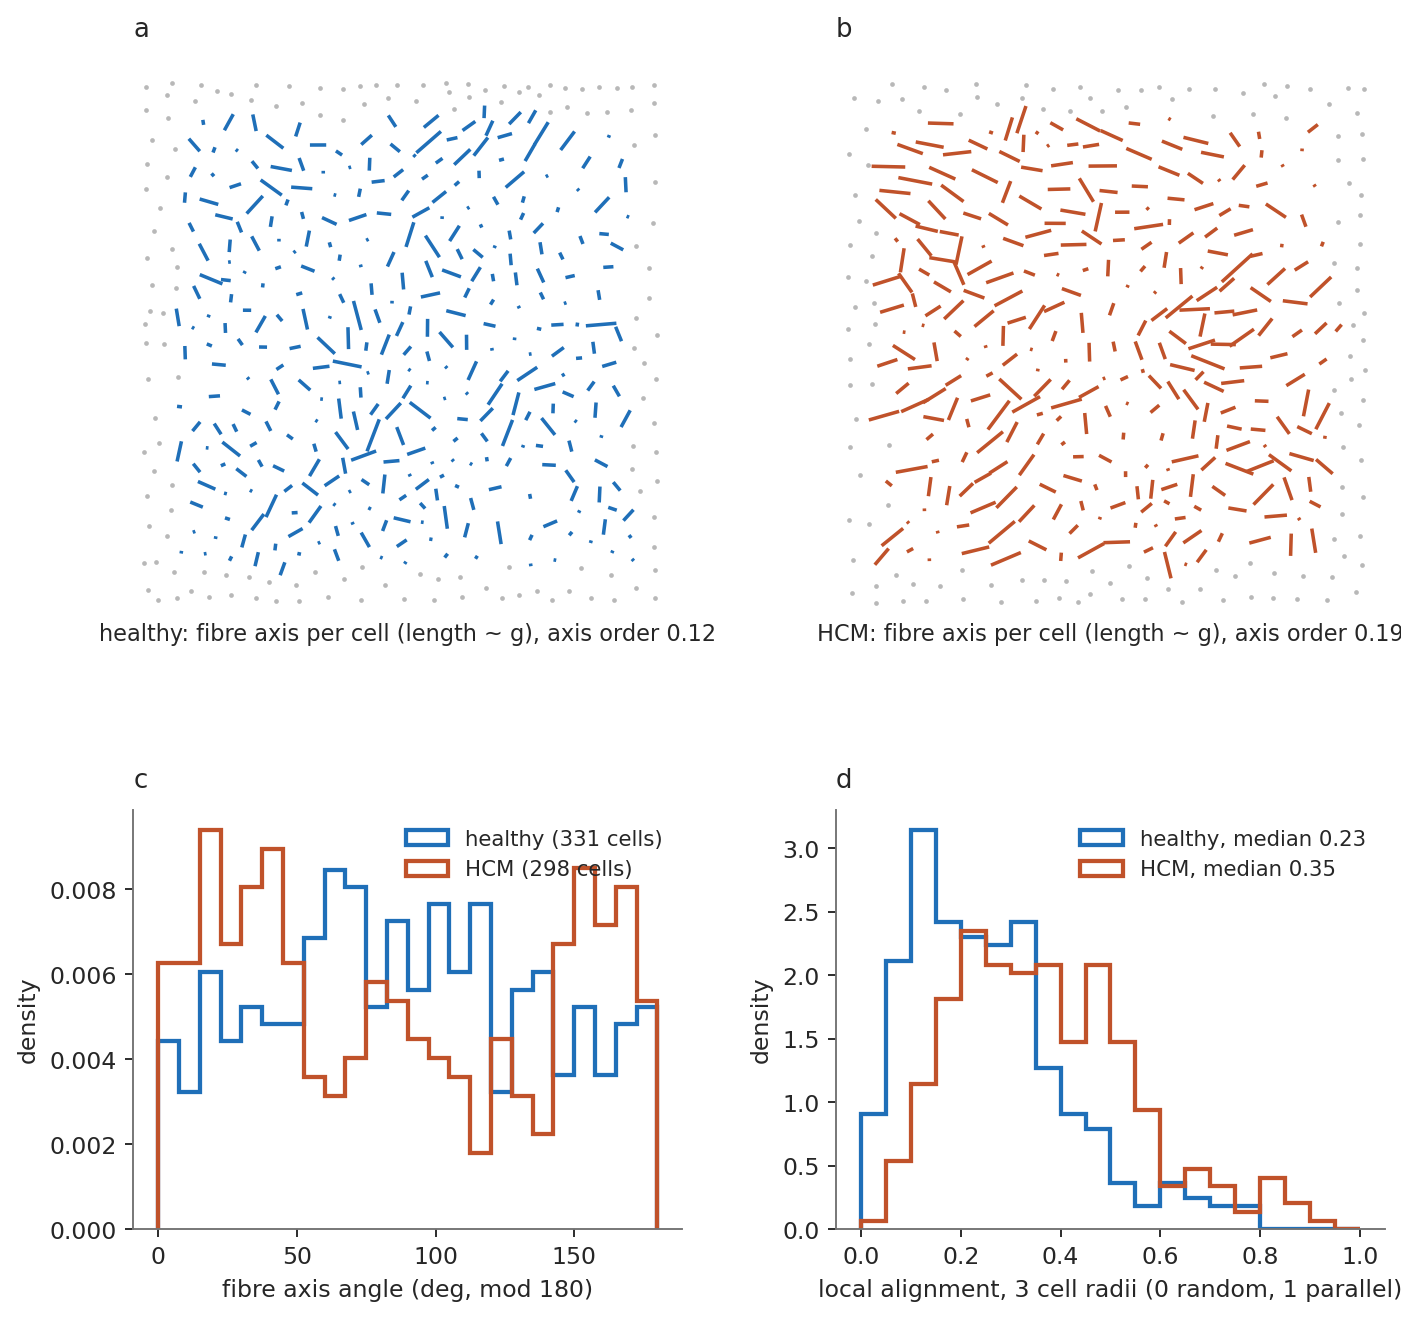
\includegraphics[width=0.74\linewidth]{figures/fig_axes.png}
\caption{Fibre axes. (a, b) One line per interior cell along $\varphi_j$, length $\propto g_j$; grey dots
the band cells. (c) Axis angle. (d) Local alignment: $|\langle e^{2i\varphi}\rangle|$ over the neighbours
within three cell radii (0 random, 1 parallel).}
\label{fig:axes}
\end{figure}

\begin{table}[h]
\centering\small
\begin{tabular}{@{}lcc@{}}
\toprule
 & healthy (331 cells) & HCM (298 cells) \\
\midrule
recorded peak shortening per cell, median & 0.025 & 0.040 \\
fitted $g$, median & 0.037 & 0.063 \\
fitted $g_2$, median & $-0.035$ & $-0.033$ \\
$g_2/g$ over active cells, median & $-0.70$ & $-0.48$ \\
cells with $g < 0.01$ & 19\% & 10\% \\
axis order $|\langle e^{2i\varphi}\rangle|$, whole sheet / local median (Fig.~\ref{fig:axes}d) & 0.12 / 0.23 & 0.19 / 0.35 \\
fitted $E_j$, median (engine stress units) & 236 & 222 \\
delay $\delta$, s.d. across cells & 0.079~s & 0.076~s \\
\bottomrule
\end{tabular}
\caption{The two sheets, same model, same procedure, from the fits rerun in this repository
(\code{cardio/figures\_note.py --source parity --only tables} prints these). The archived fits give the same
values to the printed digits.}
\label{tab:sheets}
\end{table}

\textbf{Discussion.} One caveat on reading Table~\ref{tab:sheets}. The recording gives motion, not force, so the fit
cannot separate a cell's stiffness from its active strain: a stiffer cell that contracts harder, or a weaker
contraction held for longer, moves the sheet the same way. We see this directly. With planted parameters the fit
recovers the active strain to 10\% of its spread but the stiffness only to 40\% (correlation 0.65), and left free on
the real data the per-cell stiffness spreads over a factor of 200, which we hold down with a prior. The pulse length
and the gain trade off in the same way. So the healthy / HCM differences in Table~\ref{tab:sheets} (fitted strain
0.037 vs 0.063, strain ratio across / along $-0.70$ vs $-0.48$, and the rest) describe one dish of each, fitted under
one choice of prior; they are not a conclusion about the two conditions.

\clearpage
%================================================================================================
\section{Install, run, demo}\label{sec:run}

\textbf{Install.} Python $\ge 3.10$, CUDA PyTorch (reference: Python 3.12.12, torch 2.9.0+cu128, numpy
2.2.6, scipy 1.16.2, tifffile 2025.10.16). From the repository root:
\begin{lstlisting}[style=sh]
pip install -e .              # torch, numpy, scipy, pyyaml, tifffile
pip install -e .[figures]     # + matplotlib (compare_sheets.py, figures_note.py)
\end{lstlisting}
\code{warp-lang} is optional (imported if present; this model names the pure-torch bodies).

\textbf{Layout.} \code{src/plexus/} the engine (13 modules, byte-identical to Plexus); \code{cardio/}
model, loader, optimiser, scorer, segmentation; \code{data/healthy}, \code{data/hcm} grid flows, labels,
label images; \code{specs/} per-beat engine specs (YAML); \code{configs/}, \code{scripts/} the recorded
flags; \code{reference/} the fits as produced; \code{tools/compare\_fits.py}; \code{PROVENANCE.md}.

\textbf{The two reporting fits} (110 and 150 min, 36 and 38 GB on an RTX A6000; fit, then scorer):
\begin{lstlisting}[style=sh]
scripts/run_healthy_allbeats.sh --device cuda:0
scripts/run_hcm_allbeats.sh --device cuda:0
\end{lstlisting}
Flags after the script name override (\code{--tag}, \code{--iters}, \code{--per-parent}, \ldots). Output in
\code{cardio/out/fits/<tag>/}: \code{fit.json} (config, per-iteration loss), \code{params.npz} (every
learnable; \code{params\_p20.npz}, \code{params\_p50.npz} at 20\% and 50\%), \code{s4\_score.json}.

\textbf{Demo} (minutes, under 4 GB): two iterations at 8 points per cell on a $48^2$ grid; a comparison
against the archived fit; the gradient check; the figures of this note.
\begin{lstlisting}[style=sh]
scripts/run_healthy_allbeats.sh --tag smoke --iters 2 --per-parent 8 --n-grid 48 --fit-frames 10 --checkpoints ''
python tools/compare_fits.py cardio/out/fits/smoke reference/healthy_allbeats
PYTHONPATH=src python cardio/fd_check.py --device cuda:0 --dtype float64 --per-parent 12 --n-grid 48 --frames 10
PYTHONPATH=src python cardio/figures_note.py --only sheets,axes
\end{lstlisting}
The smoke loss at iteration 0 is 2.0178 (reduced layout; the nominal fit starts at 1.7780); the comparison
reports its parameters as different from the reporting fit, as expected after two iterations at another
resolution. The scorer runs on any parameter file, every beat beside the replay and do-nothing baselines:
\begin{lstlisting}[style=sh]
PYTHONPATH=src python cardio/s4_score.py --params <params.npz> --specimen healthy --per-parent 120 --anchor-percell --drag 150 --fit-beats 1,2,3 --beats 1,2,3
\end{lstlisting}
\code{cardio/s4\_residual.py} splits the residual by component and time. Other scripts:
\begin{lstlisting}[style=sh]
python cardio/segmentation.py --tif <movie.ome.tif>          # rebuild the segmentation (not needed: outputs are shipped)
scripts/make_cont_overlay_particles.sh <movie.ome.tif> [fit dir]   # the continuous three-beat movie
\end{lstlisting}

\begin{thebibliography}{9}\small
\bibitem{hu2018} Hu, Y., Fang, Y., Ge, Z., Qu, Z., Zhu, Y., Pradhana, A., Jiang, C. (2018). A moving least squares
material point method with displacement discontinuity and two-way rigid body coupling. \emph{ACM Trans.\ Graph.}
37(4):150. Code: \url{https://github.com/yuanming-hu/taichi_mpm}.
\bibitem{sulsky1994} Sulsky, D., Chen, Z., Schreyer, H.~L. (1994). A particle method for history-dependent materials.
\emph{Comput.\ Methods Appl.\ Mech.\ Eng.} 118:179--196.
\bibitem{xu2025} Xu, M., Song, C.~Y., Levin, D.~I.~W., Hyde, D. (2025). A differentiable material point method
framework for shape morphing. \emph{IEEE TVCG} 31(10):9140--9153.
\end{thebibliography}

\end{document}
